\documentclass[compress,red]{beamer}
\mode<presentation>

\usetheme{PaloAlto}
% other themes: AnnArbor, Antibes, Bergen, Berkeley, Berlin, Boadilla, boxes, CambridgeUS, Copenhagen, Darmstadt, default, Dresden, Frankfurt, Goettingen,
% Hannover, Ilmenau, JuanLesPins, Luebeck, Madrid, Maloe, Marburg, Montpellier, PaloAlto, Pittsburg, Rochester, Singapore, Szeged, classic

%\usecolortheme{lily}
% color themes: albatross, beaver, beetle, crane, default, dolphin, dov, fly, lily, orchid, rose, seagull, seahorse, sidebartab, structure, whale, wolverine

%\usefonttheme{serif}
% font themes: default, professionalfonts, serif, structurebold, structureitalicserif, structuresmallcapsserif

% pdf is displayed in full screen mode automatically
%\hypersetup{pdfpagemode=FullScreen}

% define your own colours:
\definecolor{Red}{rgb}{1,0,0}
\definecolor{Blue}{rgb}{0,0,1}
\definecolor{Green}{rgb}{0,1,0}
\definecolor{magenta}{rgb}{1,0,.6}
\definecolor{lightblue}{rgb}{0,.5,1}
\definecolor{lightpurple}{rgb}{.6,.4,1}
\definecolor{gold}{rgb}{.6,.5,0}
\definecolor{orange}{rgb}{1,0.4,0}
\definecolor{hotpink}{rgb}{1,0,0.5}
\definecolor{newcolor2}{rgb}{.5,.3,.5}
\definecolor{newcolor}{rgb}{0,.3,1}
\definecolor{newcolor3}{rgb}{1,0,.35}
\definecolor{darkgreen1}{rgb}{0, .35, 0}
\definecolor{darkgreen}{rgb}{0, .6, 0}
\definecolor{darkred}{rgb}{.75,0,0}

\xdefinecolor{olive}{cmyk}{0.64,0,0.95,0.4}
\xdefinecolor{purpleish}{cmyk}{0.75,0.75,0,0}

% \usepackage{beamerinnertheme_______}
% inner themes include circles, default, inmargin, rectangles, rounded

%\usepackage{beamerouterthemesmoothbars}
% outer themes include default, infolines, miniframes, shadow, sidebar, smoothbars, smoothtree, split, tree

%\useoutertheme[subsection=false]{smoothbars}

% to have the same footer on all slides
%\setbeamertemplate{footline}[text line]{xxx xxx xxx}
%\setbeamertemplate{footline}[text line]{} % or empty footer

% include packages
%\usepackage[normal]{subfigure}
\usepackage{multicol}
\usepackage{amssymb,amsmath,amsfonts}
\usepackage{epsfig}
\usepackage{graphicx}
\usepackage[all,knot]{xy}
\xyoption{arc}
\usepackage{url}
\usepackage{multimedia}
\usepackage{hyperref}
\usepackage{setspace}
\usepackage{hyperref}
%\usepackage{booktabs}
%\usepackage[table]{xcolor}
% below are packages that i had included in the paper
\usepackage[english]{babel}
%\usepackage{cite}
%\usepackage{acronym}
%\usepackage{bibentry}
%\usepackage[normal]{subfigure}
%\nobibliography*

%to have option to comment some parts of the text
%\usepackage{comment}

\title{What is Tech? Data Science}
%\subtitle{}
\author{Tatjana Predojev}
\institute{\href{mailto:tatjanapredojev@gmail.com}{tatjanapredojev@gmail.com} }

\date{\scriptsize Women Who Code, February 2017}

\begin{document}

\frame{
\titlepage
}

\setcounter{tocdepth}{1}

% \newpage
% \tableofcontents
% \include{Section1_Whatis}
% \include{Section2_Wherestart}
% \include{Section3_Getexp}
% \include{Section4_Conclusion}

\section{What is Data Science?}
\frame{\frametitle{What is data science?}

\begin{exampleblock}{}
 {"Data Scientist (n.): someone who is better at statistics than any software engineer and better at software engineering than any statistician."} \\
  \hspace*\fill{Josh Wills on twitter, 2012}
\end{exampleblock}
\vspace{0.3cm}
\centering{\Large No consensus about the correct definition!}
\vspace{0.3cm}

\begin{itemize}
 \item Tech end
 \begin{itemize}
  \item machine learning (python, R), Big Data (Spark, \textcolor{Blue}{\href{http://www.h2o.ai/}{h20}}), very technical (computer scientists)
 \end{itemize}
 \item Business end
 \begin{itemize}
  \item Excel, SAS, SPSS, lots of visualisation (Tableau, QlickView), less technical
 \end{itemize}
\end{itemize}
}
% variants in between
% tech: (mostly) startups, business: banks, consulting agencies

\frame{\frametitle{Good news}
\begin{itemize}
 \item New field for everyone
 \begin{itemize}
  \item goes beyond statistics (a lot more programming-oriented)
 \end{itemize}
 \vspace{1cm}
 \item Funny example: Spark initially released in 2012 vs. job ads requirements (at least five years experience in Spark)
\end{itemize}
}

\section{Where to start?}
\frame{\frametitle{Where to start?}
\begin{itemize}
 \item Love maths :)
 \item Free online course \emph{Machine Learning} by Andrew Ng 
 % cross-validation to select the model and estimate error
 \item Another free course \emph{Statistical Learning} by Hastie and Tibshirani
 \begin{itemize}
  \item download free books both Intro and Elements
 \end{itemize}
 \item Cloudera's free \href{https://www.udacity.com/course/intro-to-hadoop-and-mapreduce--ud617}{\emph{\textcolor{Blue}{Intro to Hadoop \& MapReduce}}} hosted by Udacity 
 \item \emph{Algorithms} by Robert Sedgewick hosted by coursera
\end{itemize}
}

\section{Get experience}
\frame{\frametitle{Get some experience!}
\begin{itemize}
 \item My story: management consulting and tech startup
 \item On a regular workday: read scientific papers, \textcolor{darkred}{understand algorithms}, ``get your hands dirty'' i.e. code, improve method accuracy, improve performance, understand and interpret results
 \item Normally, machine learning algorithms are not implemented directly, but applied (lots of pre- and post-processing)
\end{itemize}
}

\frame{\frametitle{Practice!}
\begin{itemize}
 \item Practice with \textcolor{darkred}{open data}
 \begin{itemize}
  \item example: Renfe train schedules and delays
 \end{itemize}
 \vspace{1cm}
 \item Kaggle: form a team
 \begin{itemize}
  \item protip: install Anaconda for package version hell
 \end{itemize}
\end{itemize}
}

\section{Conclusion}
\frame{\frametitle{}
\centering{\Large Sexiest job of the 21st century?}
\vspace{1.5cm}
\begin{itemize}
 \item Choose what you genuinely like doing, irrespective of the buzz
\end{itemize}
}

\frame{\frametitle{Thank you!}
\begin{figure}[tbp!]
\centering{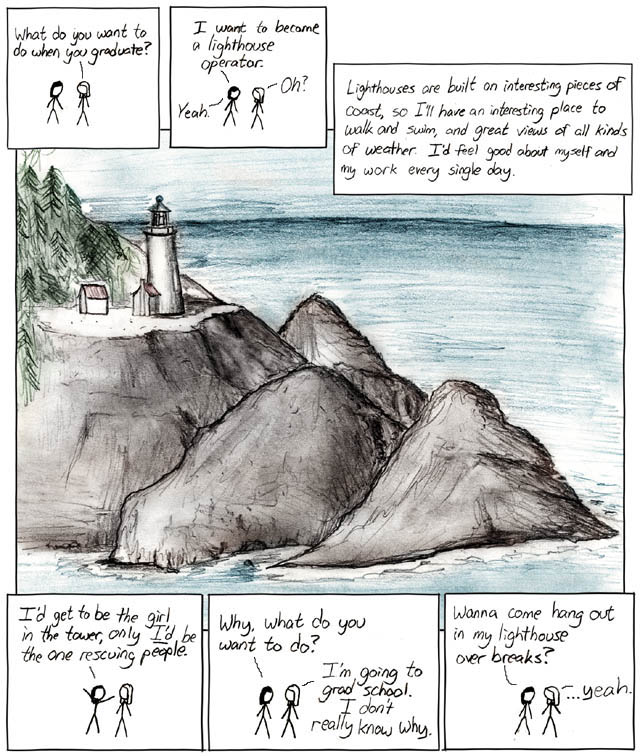
\includegraphics[height=0.9\textheight]{graduation.jpg}}
\end{figure}
}

\end{document}
